\pagenumbering{arabic}
\section{功能测试}
本测试由用例生成测试用例.具体生成步骤为:
\begin{enumerate}
	\item 进行用例建模;
	\item 根据用例, 确定基本流和各备选流;
	\item 根据基本流及备选流来确定各个由它们构成的测试场景;
	\item 由各个场景设计构造测试用例矩阵.
\end{enumerate}


\subsection{用例建模}
\begin{figure}[thbp!]
	\centering
	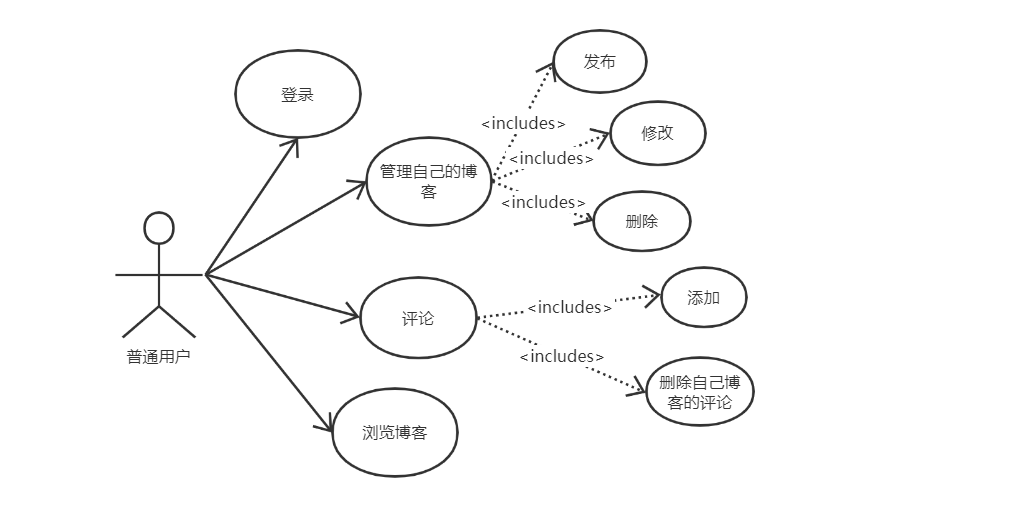
\includegraphics[width=0.8\linewidth]{figure/use_case}
	\caption{用户用例图}
%	\label{fig:IMG_1832}
\end{figure}
\subsection{基本流及备选流}
基本流如下:
\begin{table}[thbp!]
	\centering
	\begin{tabular}{|l|l|}
		\hline
		基本流 & \begin{tabular}[c]{@{}l@{}}本用例的开端是用户已经进入博客站点.\\ \\ 1. 登录账户 - 用户输入账户及密码后,网页状态切换为登陆状态,显示用户主页.
		\\ 2. 博客操作 - 进行博客浏览、评论、博客管理等操作.	\\ 3. 退出账户 - 用户选择退出则切换为游客状态;或者用户直接退出浏览页面,系\\统保存token以等待下次访问.
		\end{tabular} \\ 
		\hline
	\end{tabular}
\end{table}
备选流如下:
\begin{table}[thbp!]
	\centering
	\begin{tabular}{|l|l|}
		\hline
		\begin{tabular}[c]{@{}l@{}}备选流1\\ 用户密码输入错误\end{tabular} & 在基本流步骤1中 - 如果用户账号或密码输入错误,将反复进行提醒.                                                                                      \\ \hline
		\begin{tabular}[c]{@{}l@{}}备选流2\\ 用户浏览文章\end{tabular}   & \begin{tabular}[c]{@{}l@{}}在基本流步骤2中 - 如果用户进入主页后,\\   \quad{}点击主页文章即进入浏览\\ \quad{}文章事件流.点击退出或者关闭浏览页面则加入基本流3.\end{tabular}             \\ \hline
		\begin{tabular}[c]{@{}l@{}}备选流3\\ 用户修改文章\end{tabular}   & \begin{tabular}[c]{@{}l@{}}在备选流步骤2中 - 如果文章是用户自己发布的文章,\\   \quad{}文章下方点击修改,即进入备选流3的文章修改页面.点击发布\\\quad{}或退出修改页面则 回到备选流2.\end{tabular} \\ \hline
		\begin{tabular}[c]{@{}l@{}}备选流4\\ 用户删除文章\end{tabular}   & \begin{tabular}[c]{@{}l@{}}在备选流步骤2中 - 如果用户浏览的文章为自己发布文章,\\   \quad{}则跳出是否确认删除文章的弹窗.确认删除文章后则回到备选流2.\end{tabular}                \\ \hline
		\begin{tabular}[c]{@{}l@{}}备选流5\\ 用户评论文章\end{tabular}   & \begin{tabular}[c]{@{}l@{}}在备选流步骤2中 - 如果用户在评论框输入内容并点击发布,\\   \quad{}则会在文章下方留下相应评论.随后回到备选流2继续文章浏览.\end{tabular}                \\ \hline
		\begin{tabular}[c]{@{}l@{}}备选流6\\ 用户删除评论\end{tabular}   & \begin{tabular}[c]{@{}l@{}}在备选流步骤2中 - 如果用户在文章下方的评论为自己发布的,\\   \quad{}则可以选择删除.随后回到备选流2.\end{tabular}                           \\ \hline
	\end{tabular}
\end{table}
\subsection{测试场景}
由基本事件流及备选事件流,得出以下测试场景:
%\clearpage
\begin{table}[thbp!]
	\centering
	\begin{tabular}{|l|l|l|l|l|}
		\hline
		场景1  & 基本流 &      &      &      \\ \hline
		场景2  & 基本流 & 备选流1 &      &      \\ \hline
		场景3  & 基本流 & 备选流2 &      &      \\ \hline
		场景4  & 基本流 & 备选流2 & 备选流3 &      \\ \hline
		场景5  & 基本流 & 备选流2 & 备选流4 &      \\ \hline
		场景6  & 基本流 & 备选流2 & 备选流5 &      \\ \hline
		场景7  & 基本流 & 备选流2 & 备选流6 &      \\ \hline
		场景8  & 基本流 & 备选流1 & 备选流2 &      \\ \hline
		场景9  & 基本流 & 备选流1 & 备选流2 & 备选流3 \\ \hline
		场景10 & 基本流 & 备选流1 & 备选流2 & 备选流4 \\ \hline
		场景11 & 基本流 & 备选流1 & 备选流2 & 备选流5 \\ \hline
		场景12 & 基本流 & 备选流1 & 备选流2 & 备选流6 \\ \hline
	\end{tabular}
\end{table}
\subsection{测试用例矩阵}
由以上测试场景,构造出以下用例矩阵:

\begin{table}[thbp!]
	\centering
	\resizebox{\textwidth}{!}{
	\begin{tabular}{|l|l|c|c|l|l|}
		\hline
		\textbf{测试用例ID号} & \textbf{场景/条件}     & \multicolumn{1}{l|}{\textbf{账号}} & \multicolumn{1}{l|}{\textbf{密码}} & \textbf{文本框输入} & \textbf{预期结果}               \\ \hline
		\textbf{CW1}     & 场景1 - 成功登录与退出      & √                                & √                                & 无              & 成功退出博客站点或本地保存token.         \\ \hline
		\textbf{CW2}     & 场景2 - 任意次账户或密码输入有误 & |                                & |                                & 无              & 跳出错误提示窗口,关闭后返回登录页.          \\ \hline
		\textbf{CW3}     & 场景3 - 登录后浏览博客文章    & √                                & √                                & 无              & 正确显示博客文章分页,点击后显示详细内容.       \\ \hline
		\textbf{CW4}     & 场景4 - 对博客文章进行修改    & √                                & √                                & 非空字符           & 提交修改并跳转同步后文章页面.             \\ \hline
		\textbf{CW5}     & 场景4 - 对博客文章进行不合法修改 & √                                & √                                & 空字符            & 跳出错误提示窗口,若退出则不同步修改.         \\ \hline
		\textbf{CW6}     & 场景5 - 对博客文章进行删除    & √                                & √                                & 无              & 对文章列表对应条目进行删除并返回同步后的分页界面.   \\ \hline
		\textbf{CW7}     & 场景6 - 对博客文章进行评论    & √                                & √                                & 非空字符           & 动态刷新评论区并将评论字段变化同步至数据库.      \\ \hline
		\textbf{CW8}     & 场景6 - 对博客文章进行不合法评论 & √                                & √                                & 空字符            & 跳出错误提示弹窗.                   \\ \hline
		\textbf{CW9}     & 场景7 - 对用户自己的评论进行删除 & √                                & √                                & 无              & 对文章页面动态刷新,并删除数据库文章对应评论字段成员. \\ \hline
		
		%%=============
		
		
		\textbf{CW10}     & 场景8 - 登录后浏览博客文章    & √                                & √                                & 无              & 正确显示博客文章分页,点击后显示详细内容.       \\ \hline
		\textbf{CW11}     & 场景9 - 对博客文章进行修改    & √                                & √                                & 非空字符           & 提交修改并跳转同步后文章页面.             \\ \hline
		\textbf{CW12}     & 场景9 - 对博客文章进行不合法修改 & √                                & √                                & 空字符            & 跳出错误提示窗口,若退出则不同步修改.         \\ \hline
		\textbf{CW13}     & 场景10 - 对博客文章进行删除    & √                                & √                                & 无              & 对文章列表对应条目进行删除并返回同步后的分页界面.   \\ \hline
		\textbf{CW14}     & 场景11 - 对博客文章进行评论    & √                                & √                                & 非空字符           & 动态刷新评论区并将评论字段变化同步至数据库.      \\ \hline
		\textbf{CW15}     & 场景11 - 对博客文章进行不合法评论 & √                                & √                                & 空字符            & 跳出错误提示弹窗.                   \\ \hline
		\textbf{CW16}     & 场景12 - 对用户自己的评论进行删除 & √                                & √                                & 无              & 对文章页面动态刷新,并删除数据库文章对应评论字段成员. \\ \hline
		
	\end{tabular}

}
	
\end{table}



















